\documentclass{article}
\usepackage[margin=1in]{geometry}
\usepackage{amsmath,amsthm,amssymb}
\usepackage{bbm,enumerate,mathtools}
\usepackage{tikz,pgfplots}
\usepackage{chessboard}
\usepackage[hidelinks]{hyperref}
\usepackage{multicol} % Problem 35

\newenvironment{question}{\begin{trivlist}\item[\textbf{Question.}]}{\end{trivlist}}
\newenvironment{note}{\begin{trivlist}\item[\textbf{Note.}]}{\end{trivlist}}
\newenvironment{references}{\begin{trivlist}\item[\textbf{References.}]}{\end{trivlist}}
\newenvironment{related}{\begin{trivlist}\item[\textbf{Related.}]\end{trivlist}\begin{enumerate}}{\end{enumerate}}


\begin{document}
\rating{4}{2}
Consider convex polygons with integer coordinates. The notion of a best
Diophantine approximation can be generalized to equilateral triangles by
saying that a triangle is a better diophantine approximation if
the ratio of the largest side to the smallest side is less than the ratio of
any other triangle with smaller perimeter.
\begin{figure}[ht!]
  \centering
  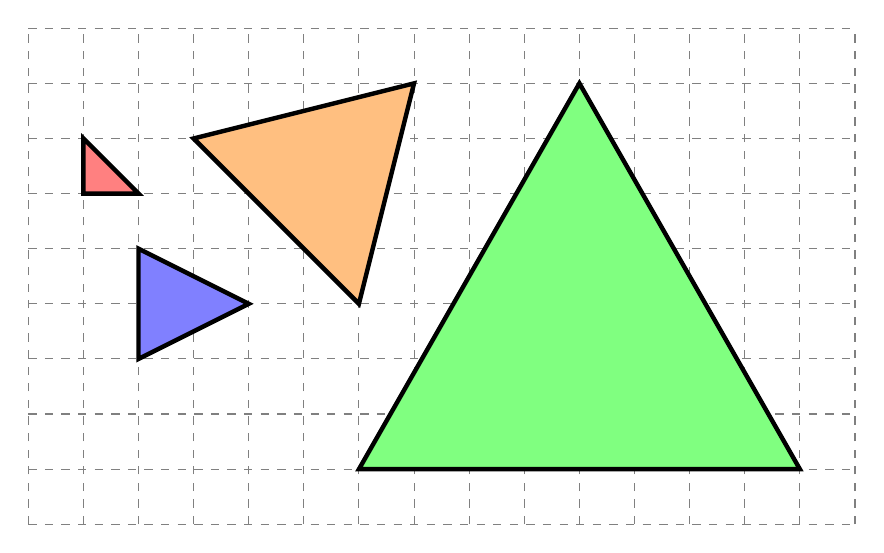
\begin{tikzpicture}[scale=0.7]
    \draw[gray, dashed] (0,0) grid (15,9);
    \draw[ultra thick, fill=red!50] (1,6)--(2,6)--(1,7)--cycle;
    \draw[ultra thick, fill=blue!50] (2,5)--(2,3)--(4,4)--cycle;
    \draw[ultra thick, fill=orange!50] (6,4)--(3,7)--(7,8)--cycle;
    \draw[ultra thick, fill=green!50] (6,1)--(14,1)--(10,8)--cycle;
  \end{tikzpicture}
  \caption{
    Four best (?) Diophantine approximations of an equilateral triangle.
    The red triangle has a ratio of $\sqrt{2/1} \approx 1.41$,
    the blue has a ratio of $\sqrt{5/4} \approx 1.118$,
    the orange has a ratio of $\sqrt{18/17} \approx 1.029$, and
    the green has a ratio of $\sqrt{64/63} \approx 1.008$.
  }
\end{figure}
\begin{question}
  What is the growth of the perimeter of the $k$-th best Diophantine
  approximation of an equilateral triangle as a function of $k$?
\end{question}

\begin{related}
  \item How can this be generalized in a reasonable way to regular $n$-gons?
    (Just looking at side lengths isn't enough---angles can behave badly.)
  \item What if this is done on tetrahedra?
\end{related}
\begin{references}
  \item \url{https://math.stackexchange.com/q/2251555/121988}
  \item \url{https://en.wikipedia.org/wiki/Near-miss_Johnson_solid}
\end{references}
\end{document}
